\chapter{Metodología}

\section{Datos empleados}

Los datos empleados en este estudio representan la información local del nivel del mar en la zona costera de Buenaventura y la información espacial en el Pacífico tropical, se describen a continuación:

a) Datos de mareógrafo: En la bahía de Buenaventura  se han captado registros del nivel del mar mediante un mareógrafo ubicado en 3.8906 \textdegree N, -77.0808 \textdegree W. El principio físico que usa un mareógrafo es la transmisión de un haz electromagnético hacía la superficie libre con una frecuencia modulada y el retorno de dicha señal bajo el efecto doppler que permite determinar la distancia existente entre el transmisor y la superficie libre. Los errores que se pueden obtener bajo este método son debidos a cambios en la temperatura del aire, la interferencia de objetos en el haz e inclusive a la acción de las olas \citep{UNESCO2016}. Este mareografo hace parte de la red de estaciones del nivel del mar creada por la comisión oceanográfica intergubernamental de la UNESCO y sus registros del nivel del mar están disponibles desde 1953 hasta 2014, a resolución horaria. Debido a operaciones de mantenimiento y reparación, existen datos faltantes a largo del registro que han generado problemas en el tratamiento de la información explicados posteriormente (fig \ref{fig:serie_real}). La información está disponible en la página web \url{www.ioc-sealevelmonitoring.org}.

\begin{figure}[H]
	\centering
	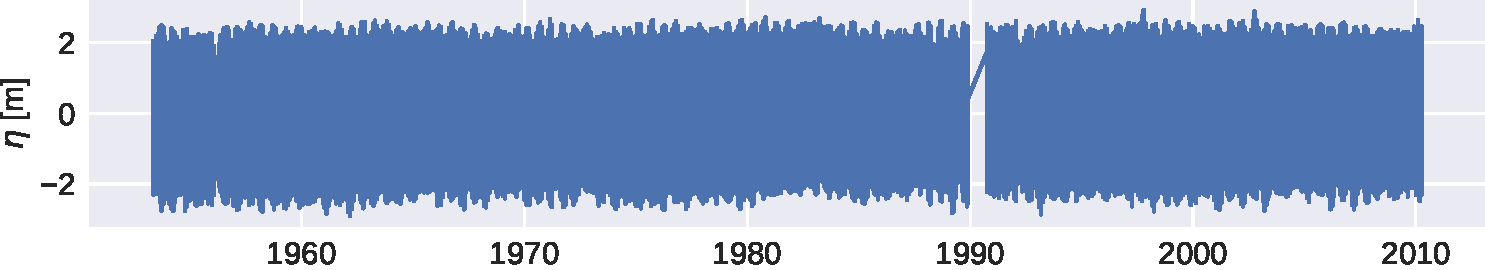
\includegraphics[width=\textwidth]{serie_mareografo.pdf}
	\caption{Serie de nivel del mar capturada por el mareógrafo de Buenaventura}
	\label{fig:serie_real}
\end{figure}

b) Datos de reanálisis: Diferentes centros de análisis de información meteorologíca y oceánica como el Centro Europeo para pronósticos meteorlógicos de medio alcance y el Servicio de Monitoreo del Medio Marino de Copérnico (ECFMW y CMEMS por sus siglas en inglés respectivamente), desarrollan y ejecutan diferentes modelos para describir la evolución espacio-temporal de variables termodinámicas como temperatura, salinidad, concentración de hielo, nivel del mar, etc. CMEMS usó el modelo de circulación global oceánica NEMO en conjunto con técnicas de reanálisis para generar un producto llamado GLORYS12V1, allí se puede obtener información del nivel del mar a partir de datos altimétricos desde 1993 hasta 2018 \citep{Fernandez2018}. La resolución espacial es de 1/12\textdegree x 1/12\textdegree y la resolución temporal es mensual. La región de descarga está comprendida entre -10\textdegree N y 10\textdegree N y entre 130\textdegree E y -74\textdegree
W. La información está disponible en la página web \url{marine.copernicus.eu}.

\section{Análsis exploratorio de los datos}

Con la serie del mareógrafo, se realiza la  descomposición armónica de la marea, sin embargo, al tener años con hasta 80\% de datos faltantes la herramienta T\_TIDE no estima bien la amplitud de los armónicos más importantes, así que se emplearon dos alternativas: a) el uso de los 18.6 años más completos dentro de la serie, debido al ciclo nodal lunar y b) el uso del mayor período de registro continuo (6 años). En esta última se debía extrapolar la información de las componente de corto plazo para todo el registro y asumir la pérdida de información de las componentes que sólo ocurren en el largo plazo. Finalmente, ninguna de las dos generó buenas descomposiciones armónicas, y se decidió usar un herramienta más reciente, PyTides \citep{Schuremann1958}.

Restando la marea astronómica de la serie medida por el mareógrafo se obtiene la serie de marea residual, se calculó su valor medio para restarlo a toda la serie para determinar finalmente la \textbf{serie de nivel medio del mar}

Paralelo al tratamiento de la información del mareógrafo, se determinan las series de nivel medio del mar para cada uno de los píxeles de la región dónde se descargo la información espacial del nivel. El proceso empleado es similar al descrito en el parrafo anterior, la resta del valor medio a toda la serie.

\section{Caracterización del nivel del mar durante eventos ENSO}

Se grafican las sobrelevaciones y descensos del nivel del mar suavizadas en ventanas de 3 meses junto a los períodos de tiempo dónde se presentaron fases cálidas y frías del ENSO seǵun el índice ONI, esto con el objetivo de conocer su comportamiento durante esos meses. También se comparó la serie mensual del nivel del mar suavizada en ventanas de 3 meses con el valor directo del índice

Con las series de sobrelevaciones y descensos diarios del nivel se caracterizan los eventos Niño y Niña ocurridos desde 1953 hasta 2010 en términos de su duración y sobrelevación/descenso ocurrido. Dado que se presume que los aumentos/descesos del nivel del mar se pueden ver agravados por la duración de los eventos ENSO y que ondas océanicas Kelvin con períodos de 3 meses pueden modular dichos cambios \citep{Fedorov2019}, los eventos Niño y Niña se clasificaron en períodos de 90-180 días, 180-360 días y mayores a 360 días 

Con la información del CMEMS, se grafica un diagrama de Hovmöller para conocer la evolución temporal de las sobrelevaciones del nivel del mar durante las fases cálidas y frías del ENSO y compararla con la información mensual del mareógrafo.

\section{Efecto del ENSO en la variabilidad del nivel del mar}
	
Para estudiar el aporte del ENSO en la variabilidad del nivel del mar, se analiza la escala interanual a través de dos procedimientos diferentes. Por un lado, para cada píxel, se filtra la serie de nivel medio del mar en la banda de interés del espectro de potencias de Fourier, definida entre 2 años y 6 años. Posteriormente se emplean análisis de componentes principales (PCA por sus siglas en inglés) \citep{Lund2000} y se selecciona la componente principal que más aporta a la varianza junto con su modo de oscilación temporal. Finalmente, se compara esa componente principal con un índice macroclimático del ENSO, en este caso, el índice ONI.

Por otro lado, se calcula para cada píxel, la varianza total y la varianza asociada a la banda de interés especificada anteriormente y con ello, se determinan los mapas de varianza, varianza en la banda y porcentaje de varianza. Estos mapas permiten identificar las regiones dónde la varianza en la escala interanual aporta más o menos a la varianza total.

\section{Predicción del nivel del mar en una zona costera de interés}\label{sec:1}

Se determina una región costera frente a la bahía de Buenaventura para predecir su serie de nivel del mar \citep{Montagut2012}. Su ubicación está entre -3.65\textdegree N y 3.85\textdegree N y entre -77.6\textdegree W y -77.2\textdegree W, después se promedia espacialmente el nivel medio del mar para obtener una serie representativa, usada posteriormente en correlaciones con otras regiones del océano.

A fin de encontrar una región que permita pronosticar el comportamiento del nivel del mar en la zona costera elegida en el literal anterior, se realizan mapas para toda la región dónde en cada píxel se calcula la correlación de Spearman entre la serie representativa de la zona costera rezagada 1, 2 y 3 meses y las series de nivel del mar, temperatura, velocidad de las corrientes en la longitud y velocidad de las corrientes en la latitud. Para cada variable, se obtuvo diferentes zonas dónde se presentaron las mayores correlaciones y en ellas se realizó un promedio espacial para obtener las series que funcionen como predictoras del nivel del mar en la zona costera.

Finalmente, se construyó y entrenó una red neuronal artificial con la función tangente hiperbólica como función de activación y con \textbf{corrección del sesgo}, se filtraron las series de todas las variables en la banda de espectral de 2 a 6 años y adicionalmente, para optimizar las predicciones en la zona costera a partir de las series de las variables predictoras en las regiones mar afuera respectivas, se escalaron las series entre -1 y 1 y se evaluaron las redes más óptimas, así como los pesos que asignaban a las diferente conexiones entre los nodos de cada capa, se eligió una configuración específica que presentó la mayor correlación con los datos de validación.

